\chapter{章名 不要加章节序号}

\section{小节名}

使用空行分段

使用equation环境或align环境添加公式, 公式引用统一使用\emph{eqn:序号}的格式, 序号按照课本序号使用

\begin{equation}\label{eqn:1.1}
    x^2+y^2=z^2
\end{equation}

\emph{强调使用emph命令}

使用mqty命令添加矩阵:

\begin{equation}\label{eqn:1.2}
    \mqty(1&2&3\\2&3&4\\3&4&5)
\end{equation}

使用cases环境添加大括号方程组

\begin{equation}
    \begin{cases}
        x+y=2\\
        2x+y=3
    \end{cases}
\end{equation}

\subsection{子小节}

对于不需要添加编号的公式, 使用equation*或align*环境

使用figure环境与includegraphics命令添加图片(通过调整width确保图片完整显示), 引用标签使用"fig:名字"的格式

\begin{figure}
    \centering
    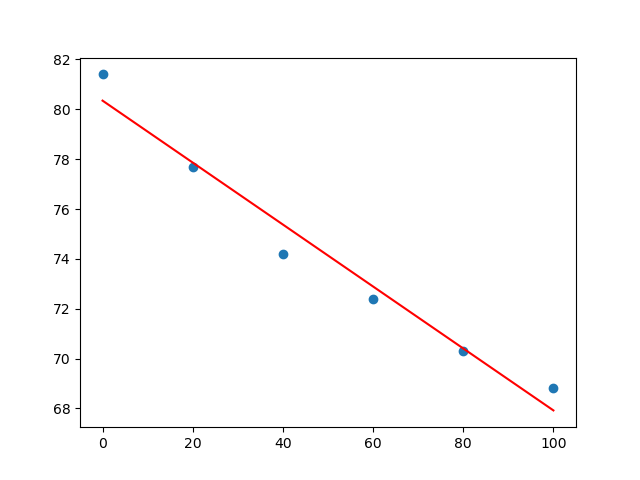
\includegraphics[width=0.7\linewidth]{Chapter3/graph/python/Figure3-1.png}
    \caption{演示}
    \label{fig:演示}
\end{figure}

\subsubsection{子子小节}

使用下述方式添加公式:

\begin{lstlisting}
# 程序实现的功能 Exercisex-x.py
import numpy as np

print("Hello World!")
\end{lstlisting}